\documentclass{standalone}
\usepackage{tikz}
\usepackage{amsmath}

\begin{document}

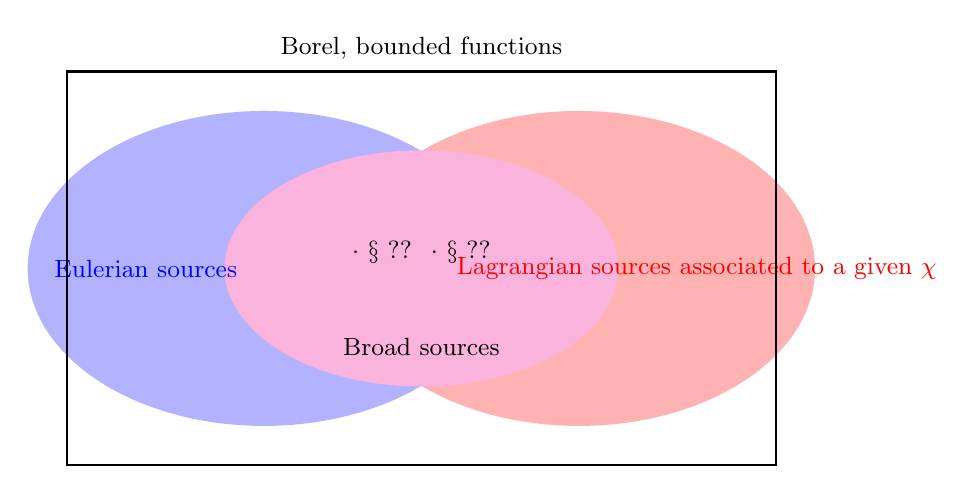
\begin{tikzpicture}
    % Set up the styles
    \tikzstyle{every node}=[font=\small]
    \tikzstyle{venn circle}=[draw,fill opacity=0.3,line width=1pt]

    % Draw the Eulerian sources circle
    \fill[blue!30] (-2,0) ellipse (3 and 2);

    % Draw the Lagrangian sources circle
    \fill[red!30] (2,0) ellipse (3 and 2);

    % Draw the overlap area
    \fill[magenta!30] (0,0) ellipse (2.5 and 1.5);

    % Draw the labels
    \node at (-3.5,0) [blue] {Eulerian sources};
    \node at (3.5,0) [red] {Lagrangian sources associated to a given $\chi$};
    \node at (0,-1) {Broad sources};

    % Add the question marks in the overlap
    \node at (-0.5,0.2) {$\cdot$ $ \mathsection$ ??};
    \node at (0.5,0.2) {$\cdot$ $ \mathsection$ ??};

    % Add the title
    \node at (0,2.8) {Borel, bounded functions};

    % Draw the outer rectangle
    \draw[thick] (-4.5,-2.5) rectangle (4.5,2.5);
\end{tikzpicture}

\end{document}